\documentclass{article}
\usepackage{hyperref}
\usepackage{graphicx}
\usepackage{float}
\usepackage{listings}
\usepackage{xcolor}

\definecolor{backcolour}{rgb}{0.95,0.95,0.92}
\lstdefinestyle{mystyle}{
    backgroundcolor=\color{backcolour},   
    basicstyle=\ttfamily\footnotesize,
    breakatwhitespace=false,         
    breaklines=true,                 
    captionpos=b,                    
    keepspaces=true,                                   
    showspaces=false,                
    showstringspaces=false,
    showtabs=false,                  
    tabsize=2
}

\lstset{style=mystyle}

\title{FHIR}
\author{Riccardo Cambianica}

\begin{document}
\maketitle
\tableofcontents
\newpage

\section{Introduzione}

\textbf{FHIR}, Fast Healthcare Interoperability Resources, è uno standard di interoperabilità sanitaria di HL7 (associazione non profit internazionale che si occupa di gestire standard per la sanità)
 che consente a una moltitudine di sistemi di scambiare informazioni sanitarie utilizzando modelli di dati concordati. In FHIR, questi modelli di dati sono semplici, diretti, contemporaneamente
leggibili da uomo e computer e, quando combinati, abbastanza robusti da trasmettere informazioni sanitarie complesse.
I core goals di FHIR sono:
\begin{itemize}
    \item Creare uno standard da utilizzare tra diverse piattaforme IT che si occupano di dati sanitari
    \item Renedere l'interoperabilità in tempo reale più semplice
\end{itemize}
In definitiva, FHIR riduce la curva d'apprendimento, rende l'interoperabilità più semplice e permette di creare in modo più veloce e semplice applicativi.

\section{Struttura di FHIR}
Il componente base di FHIR è la struttura chiamata \textbf{risorsa}. Tutto il contenuto scambiabile è definito come risorsa.
La filosofia su cui si basa lo standard FHIR è cosrtruire un set vase di risorse che, sia da sole sia combinate, possano soddisfare la maggioranza dei casi d'uso esistenti.
La modellazione FHIR usa un approccio compositivo, cioè implementa i casi d'uso combinando risorse attraverso l'uso dei loro riferimenti.
\subsection{Risorse FHIR}
In FHIR, i dati sanitari sono divisi in categorie, come ad esempio pazienti, risultati di laboratorio ed osservazioni.
Ciascuna di queste categorie è descritta approfonditamente all'interno di una risorsa FHIR, che include i suoi dati, la terminologia e altre regole che insieme formano un elemento
scambiabile.
Tutte le risorse hanno le seguenti features in comune:
\begin{itemize}
    \item un identificatore per la risorsa, tipicamente un URL che specifica dove si trova la risorsa
    \item metadati comuni
    \item un sommario in formato XHTML, facilmente leggibile
    \item un insieme di data elements, diversi per ogni tipo di risorsa
    \item un framework che permette l'estensibilità, in grado di supportare variazioni della struttura
\end{itemize}
Le istanze delle risorse possono essere rappresentate in diversi formati quali XML, JSON o RDF e attualmente esistono
157 differenti tipi di risorsa nella specifica FHIR; il progetto di stage ha approfondito in particolare la risorsa \textbf{osservazione},
che sarà presentata in seguito.
\subsection{Profili delle risorse}
La specifica base di FHIR (questa specifica) descrive un insieme di risorse di base, framework e API che vengono utilizzati in diversi contesti nel settore sanitario. Tuttavia, esiste una notevole variabilità tra le giurisdizioni e nell'ecosistema sanitario riguardo alle pratiche, ai requisiti, alle normative, all'istruzione e a quali azioni sono fattibili e/o benefiche.
Per questo motivo, la specifica FHIR è una "specifica di piattaforma" - crea una piattaforma comune o una base su cui vengono implementate diverse soluzioni. Di conseguenza, questa specifica richiede solitamente ulteriori adattamenti ai particolari contesti di utilizzo. Tipicamente, questi adattamenti specificano:
\begin{itemize}
    \item Regole su quali elementi delle risorse sono o non sono utilizzati e quali elementi aggiuntivi vengono aggiunti che non fanno parte della specifica di base
    \item Regole su quali funzionalità delle API vengono utilizzate e come
    \item Regole su quali terminologie vengono utilizzate in particolari elementi
    \item Descrizioni di come gli elementi delle risorse e le funzionalità delle API si mappano ai requisiti e/o implementazioni locali
\end{itemize}
In particolare, i \textbf{profili} sono un insieme di vincoli su una risorsa utili a definire la sua struttura.
Vengono essenzialmente utilizzati in due modi:
\textbf{Resource profiles} descritti utilizzando l'elemento "CapabilityStatement rest resource profile"
\textbf{Supported profiles} descritti utilizzando l'elemento "CapabilityStatement rest resource supportedProfile"
\subsubsection{CapabilityStatement.rest.resource.profile}
Questi profili descrivono le caratteristiche generali supportate dal sistema per ogni tipo di risorsa.
Tipicamente, questo è il superset di tutti i diversi casi d'uso implementati dal sistema.
\subsubsection{CapabilityStatement.rest.resource.supportedProfile}
Questi profili descrivono le informazioni gestite/prodotte dal sistema in base a ciascun caso d'uso. Alcuni esempi di utilizzo per questi tipi di profili sono:
\begin{itemize}
    \item Un servizio di laboratorio che produce una serie di diversi rapporti - chimica generale, emocromo, ecc. I laboratori tipici supporterebbero diverse centinaia di rapporti diversi.
    \item Un gestore delle cure che gestisce un insieme di diversi tipi di piani di cura e risorse cliniche associate.
\end{itemize}
Questi profili rappresentano diversi casi d'uso che portano a gestire le risorse del tipo indicato dal CapabilityStatement.rest.resource.type in modo diverso.
Affinché un sistema produttore e un sistema consumatore possano scambiare dati con successo basandosi su uno di questi profili supportati, non è sufficiente sapere che i sistemi hanno profili
che si sovrappongono per il caso d'uso di interesse; il consumatore deve essere in grado di filtrare l'insieme totale delle risorse messe a disposizione dal sistema produttore e gestire solo
quelle rilevanti per il caso d'uso.
Ad esempio, consideriamo un sistema di laboratorio che genera migliaia di rapporti al giorno. L'1\%  di questi rapporti è un particolare rapporto endocrinologico
che un sistema di supporto decisionale sa come elaborare. Entrambi i sistemi dichiarano di supportare il particolare profilo del rapporto endocrinologico, ma come
fa il sistema di supporto decisionale a trovare effettivamente i rapporti endocrinologici che sa come elaborare?
Una possibile opzione è che il sistema di supporto decisionale riceva ogni singolo rapporto proveniente dal sistema di laboratorio, controlli se è conforme al profilo o meno
e poi decida se elaborarlo. Verificare se una risorsa è conforme a un particolare profilo o meno è un'operazione semplice (un'opzione è utilizzare gli strumenti forniti per questo),
ma questo è un modo molto inefficiente - il sistema di supporto decisionale deve ricevere ed elaborare 100 volte più risorse di quante ne utilizzi effettivamente.
Per aiutare un consumatore a trovare l'insieme corretto di rapporti per un caso d'uso, un produttore di risorse può:
\begin{itemize}
    \item dichiarare con asserzioni di profilo documentando i profili a cui sono conformi (questo consente l'indicizzazione per profilo)
    \item cercare i profili dichiarati tramite il parametro di ricerca "profile", se il parametro di ricerca è supportato.
\end{itemize}

\subsection{Esempio istanza di una risorsa}
Di seguito è fornito un esempio di come un paziente è rappresentato come un oggetto FHIR in formato JSON.
E' possibile notare la presenza delle features descritte in precedenza.
\begin{figure}[H]
    \centering
    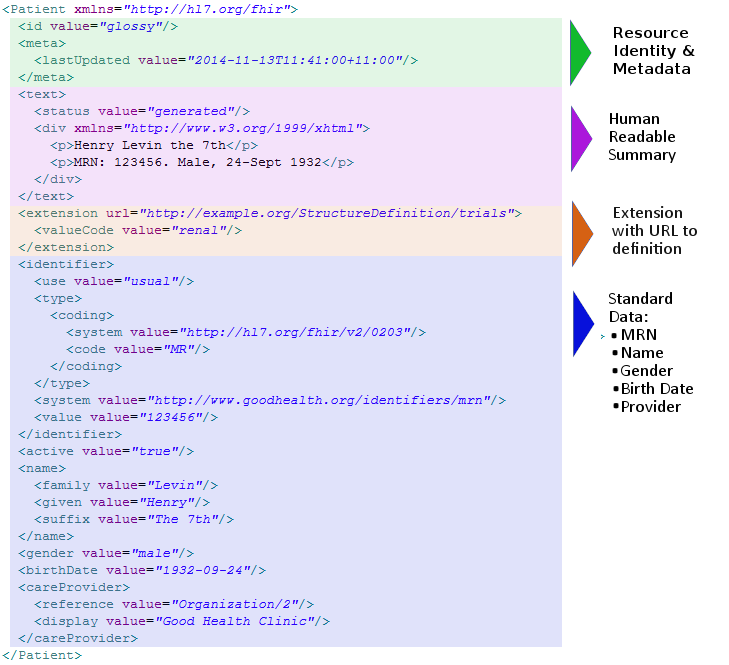
\includegraphics[width=1.35 \textwidth]{figures/esempio paziente.png}
    \label{fig:esempioPaziente}
\end{figure}
\section{Osservazione}
Le osservazioni sono un elemento fondamentale nel mondo sanitario, utili per supportare diagnosi di malattie, monitare progressi
dovuti a cure mediche o determinare pattern ricorrenti nella popolazione.
La maggioranza delle osservazioni possono essere rappresentate da coppie nome-valore coadiuvate da metadati, ma esistono anche tipi di osservazioni con strutture più complesse.
Gli usi della risorsa Osservazione sono molteplici:
\begin{itemize}
    \item Parametri vitali come pressione sanguigna, temperatura corporea o battito cardiaco
    \item Dati di laboratorio derivati da esami medici, come la quantità di glucosio nel sangue
    \item Dati risultanti dallo studio di immagini mediche, come la densità ossea o la misurazione fetale
    \item Sintomatologie cliniche
    \item Misurazioni di macchinari specifici, come elettrocardiogramma o pulsossimemtro
    \item Impostazioni di macchinari
    \item Caratteristiche fisiche personali, come ad esempio il colore dei capelli o degli occhi
    \item Storia medica familiare: malattie croniche famigliari, parenti fumatori, etc.
\end{itemize}
Tipicamente, un'osservazione riguarda il soggetto - un paziente, un gruppo di pazienti, una località o un dispositivo - e la distinzione tra il soggetto e ciò che è direttamente
misurato per un'osservazione è specificata nel codice dell'osservazione stessa (ad esempio, "Glucosio nel sangue") e non necessita di essere rappresentata separatamente.
Tuttavia, tre attributi possono essere utilizzati per rappresentare il focus dell'osservazione se non è il soggetto stesso.
\subsection{Profilare un osservazione}
Nella sua forma più semplice, un'istanza di risorsa può consistere solo di un codice, un valore e un flag di stato.
La rilevanza di altre proprietà varierà in base al tipo di osservazione.
I profili sono creati per fornire linee guida sulla cattura di determinati tipi di osservazioni per un determinato caso d'uso.
La risorsa Osservazione si concentra sul livello di dettaglio catturato dalla maggior parte dei sistemi.
Tuttavia, per un dato caso d'uso, potrebbero esserci vincoli aggiuntivi e informazioni supplementari rilevanti in determinate circostanze.
Come per altre risorse, le estensioni possono essere utilizzate per introdurre questa complessità aggiuntiva.
Lo studio del progetto di tesi ha approfondito in particolare l'area dei parametri vitali, dove c'è la necessità di un vocabolario unico
e globale per consentire un accesso e un riutilizzo onnipresenti. Questo è particolarmente vero con l'uso di dispositivi indossabili da
parte dei pazienti, dove possono/devono condividere informazioni provenienti da tali dispositivi. Per soddisfare questa necessità,
deve esistere un vocabolario coerente e una sintassi comune per raggiungere l'interoperabilità semantica.
Il profilo \textbf{FHIR Vital Signs} stabilisce le aspettative minime per la risorsa Osservazione per registrare, cercare e recuperare i segni vitali
associati a un paziente, che includono i segni vitali primari oltre a misurazioni aggiuntive come altezza, peso e BMI (Body Mass Index).
Quando un'implementazione FHIR supporta uno qualsiasi dei segni vitali elencati di seguito, l'implementazione dovrà conformarsi a questo profilo per l'osservazione dei parametri vitali.
Un'osservazione che rispetta il profilo appena descritto deve quindi avere
\begin{itemize}
    \item uno status
    \item un codice appartenente alla categoria "vital signs"
    \item un "valore magico", che descrive cosa l'osservazione sta misurando.
          A tal proposito è necessario specificare che lo standard scelto è \textbf{LOINC} per la sua diffusione capillare
    \item un paziente
    \item una data (sono accettati diversi formati) che indica quando l'osservazione è stata rilevata
    \item un valore numerico e un'unità di misura facente parte dello standard \textbf{UCUM} (Unified Code for Units of Measure)
\end{itemize}
Approfondendo il formato dei valori, è importante specificare che quando un valore di risultato è rappresentato come un concetto predefinito utilizzando un codice, viene utilizzato il datatype valueCodeableConcept (che approfondiremo nel capitolo dedicato all'implementazione).
Questo elemento è vincolato a un set di valori composto da una nomenclatura standard come SNOMED CT o da valori di risultato codificati di un sistema sorgente ("locale").
I risultati possono essere codificati in più set di valori basati su diversi sistemi di codici e questi possono essere mappati utilizzando la risorsa ConceptMap
e/o forniti come codifiche aggiuntive direttamente nell'elemento, come mostrato nell'esempio seguente.
\begin{lstlisting}
            "valueCodeableConcept": {
                "coding": [
                    {
                        "system": "http://snomed.info/sct",
                        "code": "260385009",
                        "display": "Negative"
                    }, {
                        "system": "https://acme.lab/resultcodes",
                        "code": "NEG",
                        "display": "Negative"
                    }
                ],
                "text": "Negative for Chlamydia Trachomatis rRNA"
            }
        \end{lstlisting}
\subsection{Esempio Osservazione FHIR}
\begin{lstlisting}
    {
        "resourceType": "Observation",
        "id": "body-temperature",
        "meta": {
            "profile": [
                "http://hl7.org/fhir/StructureDefinition/vitalsigns"
            ]
        },
        "text": {
            "status": "generated",
            "div": "<div xmlns=\"http://www.w3.org/1999/xhtml\"><p><b>Generated Narrative: Observation</b><a name=\"body-temperature\">"
        },
        "status": "final",
        "category": [
            {
                "coding": [
                    {
                        "system": "http://terminology.hl7.org/CodeSystem/observation-category",
                        "code": "vital-signs",
                        "display": "Vital Signs",
                        "userSelected": false
                    }
                ],
                "text": "Vital Signs"
            }
        ],
        "code": {
            "coding": [
                {
                    "system": "http://loinc.org",
                    "code": "8310-5",
                    "display": "Body temperature",
                    "userSelected": false
                }
            ],
            "text": "Body temperature"
        },
        "subject": {
            "reference": "Patient/example"
        },
        "encounter": {
            "reference": "Encounter/example"
        },
        "effectiveDateTime": "2024-05-24T10:27:02Z",
        "valueQuantity": {
            "value": 36.5,
            "unit": "C",
            "system": "http://unitsofmeasure.org",
            "code": "Cel"
        }
    }  

\end{lstlisting}
\end{document}